\begin{filecontents}{preliminary.sty}
\ProvidesPackage{preliminary}
%\DeclareOption{draft}{%
  \AtBeginDocument{%
    \renewcommand\maketitlehookc
\ProcessOptions
\RequirePackage{titling}
\endinput
\end{filecontents}

\documentclass[12pt, a4paper]{article}
\usepackage{setspace}
\usepackage{ragged2e}
\usepackage[centertags,reqno]{amsmath}
\usepackage{amssymb}
\usepackage{graphics,subfigure}
\usepackage[dvips]{graphicx}
\usepackage[dvipsnames]{xcolor}
\usepackage[hidelinks]{hyperref}
\usepackage{appendix}
\usepackage{natbib}
\usepackage{verbatim,color}
\usepackage{pdflscape}
\usepackage[showframe=false]{geometry}
\usepackage{changepage}
\usepackage{xcolor}
\usepackage{eurosym}
\usepackage{textcomp}
\usepackage[open,openlevel=1]{bookmark}
\usepackage{multirow}
\usepackage{caption}
\usepackage{hyphenat}
\usepackage{listings} % To include a Stata .do file
\usepackage{pdfpages} % To include the instructions from a pdf file
\usepackage{tikz}
\newcommand{\mybox}[2]{{\color{#1}\fbox{\normalcolor#2}}}
\doublespacing



% Exception to hyphenation
\hyphenation{par-ti-ci-pants}
\hyphenation{par-ti-ci-pant}
\hyphenation{Hy-po-the-sis}
\hyphenation{ex-pe-ri-ment}
\hyphenation{ex-pe-ri-ments}

% Allows bigger tables to be scaled down
\usepackage{adjustbox}

%From my paper with Raymond
\usepackage{tabularx,calc}
\usepackage{dcolumn}                    % Aligns tables on the decimal point
\newcolumntype{d}[1]{D{.}{.}{#1}}       %       Aligns on dot
\newcolumntype{.}{D{.}{.}{3.5}}         %       Somehow it works better
\newcolumntype{C}{@{\extracolsep{.6cm}}c@{\extracolsep{0pt}}}
\usepackage{threeparttable}
\usepackage{siunitx,booktabs}
\sisetup{
    detect-all,
    round-integer-to-decimal = true,
    group-digits             = true,
    group-minimum-digits     = 4,
    group-separator          = {\,},
    table-align-text-pre     = false,
    table-align-text-post    = false,
    input-signs              = + -,
    input-symbols            = {*},
    input-open-uncertainty   = ,
    input-close-uncertainty  = ,
    retain-explicit-plus
}

% Commands to name appendices Appendix A, Appendix B, etc.
\makeatletter
%% The "\@seccntformat" command is an auxiliary command
%% (see pp. 26f. of 'The LaTeX Companion,' 2nd. ed.)
\def\@seccntformat#1{\@ifundefined{#1@cntformat}%
   {\csname the#1\endcsname\quad}  % default
   {\csname #1@cntformat\endcsname}% enable individual control
}
\let\oldappendix\appendix %% save current definition of \appendix
\renewcommand\appendix{%
    \oldappendix
    \newcommand{\section@cntformat}{\appendixname~\thesection\quad}
}

%Adds text specifying it is a preliminary version
%\usepackage{preliminary}

\title{Testing the Elicitation Procedure \\ of the Minimum Acceptable Probability}
\author{Maria Polipciuc\thanks{Maastricht University and Vienna University of Economics and Business. Email: \url{maria.polipciuc@wu.ac.at}.} \and Martin Strobel\thanks{Maastricht University. We thank Elias Tsakas, Mats K\"{o}ster, and participants in the BEELab proposal meeting for valuable comments.}}
\date{\today	\vspace{1cm}}
\titlepage


\begin{document}
\begin{titlepage}
\clearpage
\maketitle
\thispagestyle{empty}


\begin{abstract}
%Betrayal aversion has been shown to be an important determinant of trust \citep{Bohnet2004}.
%Its original identification via Minimum Acceptable Probabilities (MAPs) allows for confounding factors to be mistaken for betrayal aversion \citep{Li2020a}.
%
%%We run an online experiment to estimate the impact of one potential confound: more pessimistic beliefs in the binary trust game compared to the control game.
%%\textcolor{red}{Participants have to state MAPs for preferring the outcome of a lottery (which will be selected at random from a set of lotteries) to a certain amount.
%%Across three treatments, the support for the lotteries is the same, but we vary the probability of each lottery to be selected.
%%--> I am thinking the text in red could be removed.}
%
%%We find that MAPs are lowest in the treatment with high mass on ``bad'' lotteries, followed by MAPs in an in-between (uniform) treatment, followed by MAPs in the treatment with high mass on ``good'' lotteries.
%In an experiment, we find that MAPs are lower the worse the prospects one faces.
%%The differences run opposite to what we expected: a lower MAP in the uniform as compared to the ``bad'' treatment.
%Underlying distributions (beliefs about them) influence valuation elicited through MAP, but in the opposite direction to the one we expected.
%This is similar to the distributional dependence of valuations elicited using the Becker--DeGroot--Marschak mechanism, which closely resembles how MAPs are elicited.

Betrayal aversion has been shown to be an important determinant of trust (Bohnet and Zeckhauser, 2004).
We study whether the way betrayal aversion is identified (as a difference in Minimum Acceptable Probabilities, MAPs) is affected by beliefs about one’s prospects.

In a within-subject design, we find that MAPs are lower the worse the prospects one faces.
This is similar to the distributional dependence of valuations elicited using the Becker–DeGroot–Marschak mechanism, of which MAPs are a special case.
Our results suggest that distributional dependence should be accounted for when eliciting MAPs to isolate betrayal aversion.

\end{abstract}
\end{titlepage}


\section{Introduction}\label{sec:intro}
Individuals have often been found to prefer exposure to a randomly generated risk than to an equiprobable risk generated by an opponent in a strategic situation.
In the context of trust games, this strategic risk premium has been dubbed \textit{betrayal aversion} \citep{Bohnet2004}.
Many papers find that betrayal aversion is an important determinant of trust \citep{Bohnet2004, Aimone2015, Fairley2016, Quercia2016, Bacine2018, Butler2018, Polipciuc2022motive}.

Betrayal aversion is identified as the difference in first mover behavior in two games: a binary trust game---a version of the trust game \citep{Berg1995} where the first mover can either send or not send an amount to the second mover---and an equivalent game where the decision at the second node is made by a random device.
If the first mover sends money, there is an efficiency gain.
Using the strategy method \citep{Selten1967}, second movers are asked whether they would return half of the (increased) amount to the first mover or keep most of it, should their matched first mover send them money.
First movers typically have to indicate their \textit{minimum acceptable probability} (MAP).
This is also elicited using a strategy-method procedure and has many features in common with the Becker--DeGroot--Marschak mechanism \citep[in short, BDM]{Becker1964}.
The MAP is a first mover's conditional threshold probability of the good outcome at the second node for preferring to send money to the second mover over the outside option (this option keeps the two players' equal initial endowments unchanged).
It is elicited without first movers knowing how many second movers (devices) chose the favorable outcome at the second node.\footnote{
The probability is calculated over the pool of second movers' decisions.
}
Then, should the threshold be reached or exceeded, first movers send money, and the outcome is decided by their matched second mover's choice (their matched device's choice).
Should the threshold not be met, the outside option is implemented.

A recent paper has shown theoretically that the elicitation procedure of MAPs used in most papers on betrayal aversion leaves the door open to potential confounds for betrayal aversion such as ``ambiguity attitudes, complexity, different beliefs, and dynamic optimization'' if players are not rational expected utility maximizers \citep{Li2020a}.
Moreover, a couple of empirical papers which use more stringent identification procedures for betrayal aversion by controlling for beliefs in the two games do not find betrayal aversion (\citeauthor{Fetchenhauer2012}, \citeyear{Fetchenhauer2012}, the second experiment in \citeauthor{Polipciuc2022inout}, \citeyear{Polipciuc2022inout}), or find it to play a role for trusting only when beliefs are far more optimistic than is generally the case \citep{Engelmann2021}.
% Maybe it makes sense to mention the next sentence after describing the similarity with BDM.
%Several papers CITE find that when dealing with complex risks, participants in experiments require an extra premium compared to simple risk aversion.
%This premium is positively correlated with ambiguity aversion. (ARE EFFECT size similar?)

In this note, we use an online experiment to measure how much of what has been called betrayal aversion is due to distributional dependence, regardless of the source of risk being random or strategic.
We remove the strategic component and show participants complete distributions over probabilities of the good (and bad) outcome of a lottery, and ask them to state their cutoff probability of the favorable outcome for preferring the lottery over a safe payoff.
Since this is a situation involving complex risk, we expect a premium between the distribution mimicking the control condition in betrayal aversion studies and the distribution mimicking the binary trust game condition, as suggested by \cite{Li2020a}.\footnote{
In both this note and in the numerical example in Appendix A in \cite{Li2020a}, the risks are quantifiable i.e. the probability distribution over lotteries is known.
Some refer to such situations as involving ambiguity, others---as involving complex risks (the compound risk of which lottery will be selected and what the outcome of the lottery will be).

Ambiguity aversion and attitudes to complex risks are positively correlated \citep{Armantier2016}.
In this paper, we refer to the situation as involving complex risk.
}
We find the opposite to be true: the higher the expected value of the probability of the favorable outcome, the higher the minimum acceptable probability required by participants to prefer the lottery.

While this is at odds with our expectations, it ties in with findings from the empirical literature on distributional dependence of willingness to pay (WTP) as elicited through the BDM mechanism.
Similarly to betrayal aversion, theoretical literature has pointed out that the BDM mechanism is not incentive compatible if players are not rational expected utility maximizers \citep{Karni1987,Horowitz2006}.
This is because individuals face uncertainty regarding the price of the good at stake and additional uncertainty about whether they will buy the good or not.
If their utility function is influenced by these uncertainties, changing the price distribution of the good might influence their valuation of the good (here, the MAP).
Several empirical papers find this to be the case for the BDM: generally, the higher the expected price of the good, the higher the WTP \citep[for a short review of this literature, see][]{Tymula2016}.
The results of \cite{Tymula2016} are partly consistent with theories of reference-dependent preferences \citep{Koszegi2006, Koszegi2007, Wenner2015}.

%The MAPs from which one identifies betrayal aversion are elicited through a variant of the Becker--Degroot--Marschak (BDM) \citep{Becker1964} mechanism, which is an often used mechanism for eliciting valuations.
%In the Becker--DeGroot--Marschak mechanism, a potential buyer states the maximum price for which she is willing to buy a good.
%A price is drawn, and if it is lower than or equal to the price she stated, she buys the good.
%If the price is higher, she keeps her endowment and does not buy the good.
%There a couple of differences between the `standard' BDM and MAP elicitation: (1) the auctioned good is a lottery, (2) instead of giving a maximum price for which they prefer the good to a safe payment, participants are asked to state a minimum probability of the favorable outcome of the lottery for which they prefer the lottery to a safe payment and (3) the underlying distribution of the probability of the favorable outcome is not (implicitly) uniform, as is the case in most studies using the distribution of potential prices for the good.


%\textcolor{red}{Here I plan to say something about possible things which may be causing the result. For this, I have to understand if two papers cited by \cite{Tymula2016}---\cite{Koszegi2006} and \cite{Wenner2015}---are relevant for our study, and what they imply for our findings.}

Our results suggest that (i) the way MAPs are elicited is sensitive to subjective beliefs, so these should be taken into account in order not to confound valuation, and (ii) the way subjective beliefs influence valuation is not in line with results of the toy model in \cite{Li2020a}.
%Further literature could explore the theoretical models which can explain why more favorable distributions raise the MAP absent strategic interaction.


The paper is structured as follows.
Section \ref{sec:proced} describes the experimental design and procedures.
Section \ref{sec:hyp} sets forth the hypothesis.
Section \ref{sec:results} presents the results.
Section \ref{sec:discussion} explains how our results inform the existing literature and suggests directions for future research.


\section{Design and procedures}\label{sec:proced}
We use a within-subject design, with each subject being exposed to all treatments sequentially.
In each treatment, participants see a graphical representation of a distribution over lotteries with two possible outcomes (a high payoff and a low payoff), but varying probabilities for each outcome.
A lottery will be drawn at random from the distribution.
This means in some treatments it is more likely to get a lottery with a high chance of a high payoff than in others.
We use three distributions over lotteries.
The distributions are ordered in terms of the expected payoff over the entire distribution, as their name suggests: the Good, the Bad, and the Uniform (the Good $>$ the Uniform $>$ the Bad).

To make the task easy to understand, we present lotteries via 32 wheels of fortune with 15 sectors each.
Dark blue sectors symbolize the high payoff (\pounds4), light blue sectors---the low payoff (\pounds1).
The sure payoff (the payoff participants receive if no wheel ends up being spun) is \pounds2.
In each treatment, participants see the wheels sorted in ascending order by the probability of the favorable outcome, with the 32 wheels equally distributed over 4 rows.
Figure \ref{fig:TheGood} below shows the distribution for the Good treatment.

\begin{figure}[h!]
  \centering
 {\includegraphics[width=\linewidth]{Left_15.pdf}}
  \caption{The Good distribution}
  \label{fig:TheGood}
\end{figure}

Two of the three distributions are meant to emulate treatments in papers on betrayal aversion.
The Uniform distribution has equal chances of occurrence for each of the possible wheels.
We assume that this is what participants expect to face in treatments with decisions made by randomization devices, unless specified otherwise.\footnote{
We assume participants in the \textit{Risky Dictator Game} in \cite{Bohnet2004} had such a distribution in mind.
}
The Bad distribution has an overall chance of a high payoff similar to the share of trustworthy respondents in papers on betrayal aversion (0.2895).
The distribution in the Good treatment mirrors the one in the Bad treatment: its overall expected chance of a high payoff is one minus that in the Bad treatment (0.7105), it has the same variance and minus the skewness of the Bad distribution.
We included this distribution to check if departures from the Uniform distribution in either direction yield effects of similar size (albeit reverse sign) on reported MAPs.
Table \ref{tab:distr} presents the distribution in each treatment as the number of wheels with X in 15 sectors yielding a high payoff (X runs from 0 to 15).


\begin{table}[htbp]
\centering \caption{The treatments: the distribution of chances (X in 15) of a high payoff}\label{tab:distr}
\begin{threeparttable}
\begin{tabular}
   {@{}
	l
	*3c
	@{}
	}
\toprule
	&	\multicolumn{3}{c}{\# of wheels with X in 15 high-payoff sectors}\\
	\cmidrule{2-4}
X 	&	{The Good}&{The Bad}&	{The Uniform}\\
\cmidrule{2-4}
0	&	1&       8&	2\\
1	&	1&       4&	2\\
2	&	1&       4&	2\\
3	&	1&       3&	2\\
4	&	1&       2&	2\\
5	&	1&       1&	2\\
6	&	1&       1&	2\\
7	&	1&       1&	2\\
8	&	1&       1&	2\\
9	&	1&       1&	2\\
10	&	1&       1&	2\\
11	&	2&       1&	2\\
12	&	3&       1&	2\\
13	&	4&       1&	2\\
14	&	4&       1&	2\\
15	&	8&       1&	2\\
\midrule
Total \# of wheels	&	32&       32&	32\\
\bottomrule

\end{tabular}
\end{threeparttable}
\end{table}

Participants are told that one of the wheels will be drawn at random, with all wheels having an equal chance to be drawn.
They are asked to state a \textit{minimum acceptable frequency} (which we refer to as MAP, even though it is not a probability, but a frequency, for easier comparison with papers on betrayal aversion): the lowest number of dark blue sectors in the randomly drawn wheel such that they prefer to spin the wheel for their payoff instead of receiving the sure payoff.\footnote{
We decided to use frequencies instead of probabilities because there is evidence that participants have an easier time expressing choice this way \citep{Quercia2016}.}
Specifically, they have to answer: ``Which wheels would you like to spin for your bonus?'' by inserting an integer between 0 and 15 in the blank space: ``I prefer to spin wheels which have at least \rule{1cm}{0.15mm} dark blue sectors.''

The experiment was conducted online using Qualtrics.
Participants were UK residents registered on a platform for conducting academic studies (Prolific).
Since the elicitation of MAPs is rather complex \citep{Quercia2016,Polipciuc2022inout}, we opted for participants who had at least a bachelor's degree.
The study was pre-registered at the AEA RCT Registry (\url{https://doi.org/10.1257/rct.7776-1.1}).

The study had three stages: a set of eliminatory comprehension questions, the three decisions, and a post-experimental questionnaire.\footnote{
In the post-experimental questionnaire, respondents answered an unincentivized question to determine their ambiguity aversion, an adapted cognitive reflection test \citep{Frederick2005,Thomson2016}, a question about the subject they studied for their most recent degree, a general risk taking question \citep{Dohmen2011}, a question about their aspiration level for earnings from participating in a survey, a couple of questions to check their anchoring susceptibility, from which an anchoring score can be computed \citep{Cheek2017}, a set of questions about their optimism/pessimism, the revised Life Orientation Test \citep{Scheier1994} and a brief sensation seeking scale, BSSS-4 \citep{Stephenson2003}.
}
Those who completed the experiment (went only through the comprehension questions) spent a median time of 12.4 (5.9) minutes and earned on average 3.96 (1) UK pounds.\footnote{
Participants were paid \pounds1 for going through the comprehension questions (regardless of the correctness of their answers).
Those who answered the comprehension questions correctly earned an additional \pounds1, \pounds2 or \pounds4 for one of their decisions.

The high average earnings of those who completed the experiment are due to a coding error which we detected after running the experiment.
Instead of decisions in all three treatments being equally likely to be selected, only those in the Good and the Uniform treatments were selected, each with equal probability.
This led all participants who had completed all stages of the experiment to have a higher chance of a higher payoff.
%This increased the payoffs of all participants who had completed the experiment.
This error should not have affected decisions, but only which decision was selected for payment.
Participants were informed about the error after the experiment.
}



\section{Hypothesis}\label{sec:hyp}
Let $p^*$ be the frequency of the high payoff, whose distribution varies between treatments.
Since we expect that attitudes towards complex risk might make participants state different MAPs in the three treatments, we adapt the toy example in \cite{Li2020a} and make the following assumptions:
\begin{itemize}
\item the utility of outcomes is fixed. We consider $U(high) = U(\pounds4) = 1$, $U(low) = U(\pounds1) = 0$, and $U(safe) = U(\pounds2) = 1/3$;\footnote{
We set the utility of the safe payoff such that $U(high) > U(safe) > U(low)$.
$U(safe) = 1/3$ is the value of the safe payoff for which a risk neutral first mover is indifferent between the lottery with these high and low payoffs, and the safe payoff.

Given our parameters (further in this section), a necessary condition for the optimal MAPs to differ in the three treatments is that $U(safe) \in [0.296, 0.516]$.
If $U(safe) \in [0.146, 0.296) \cup (0.516, 0.641]$, two of the three optimal MAPs are equal and the third one to differ.
If $U(safe) \in [0, 0.146) \cup (0.641, 1]$, all three optimal MAPs are equal.
%We set the utility of the safe payoff such that $U(\pounds2) = x \times U(\pounds4) + (1-x) \times U(\pounds1)$, where $x \in [0,1]$.
%This leads to $x^* = 1/3$.
}
\item participants use a probability weighting function because they perceive the tasks to involve complex risks. Similar to \cite{Li2020a}, we use \citeauthor{Prelec1998}'s (\citeyear{Prelec1998}) \textit{compound invariance} function:
$$w(p) = (exp(-(-ln(p))^\alpha))^\beta$$ 
\item we use $\alpha = 0.65$ and $\beta = 1.0467$, which according to \cite{Li2020a} are the most common values for risky probability weighting;
\item participants use ``forward'' evaluation: they consider the three possible outcomes and take into account their probabilities, as resulting from the probability weighting function above;
\item participants have the following rank-dependent utility function \citep{Schmeidler1989}, in which an act generated by a choice of MAP leads to:
$$RDU = w(P(\pounds4)) \times 1 + (w(P(\pounds4) + P(\pounds2)) - w(P(\pounds4))) \times (1/3)$$
where $P(\pounds4)$ is the probability of receiving the high payoff, $P(\pounds2)$ the probability of receiving the safe payoff, and $P(\pounds1)$ the probability of receiving the low payoff (which does not appear in the utility function, as the utility of the low payoff is considered to be 0).
\end{itemize}

In this case, the MAPs which maximize participants' utility in the three treatments are: $MAP_G = 7$ ($RDU = 0.628$), $MAP_U = 8$ ($RDU = 0.495$), and $MAP_B = 9$ ($RDU = 0.439$).
This leads us to expect the following ordering of MAPs:

\noindent \textbf{Hypothesis 1} \quad \textit{The MAP in the Good treatment (more mass on high values of $p^*$) is lower than the MAP in the Uniform treatment (a uniform distribution over $p^*$), which is lower than the MAP in the Bad treatment (more mass on low values of $p^*$).}

\begin{equation}
MAP_G < MAP_U < MAP_B
\end{equation}

We also consider the alternative hypothesis ($MAP_B < MAP_U < MAP_G$), which could be true if instead participants anchor on visual cues of the distributions, such as the mean.

\textcolor{red}{In Appendix \ref{section:appendixa} we discuss the implications of the assumptions we make in this section.}

\section{Results}\label{sec:results}
\subsection{The estimation sample}\label{ssec:sample}

Table \ref{tab:sample} describes the sample.
Treatment was assigned in order to balance the number of participants exposed to each of the six possible orderings of treatments.
275 of the 450 participants answered the eliminatory comprehension questions correctly and completed the experiment.
Since assignment to treatment happened before participants had gone through the comprehension questions, this leads to slightly different sizes of the subsamples for the six orderings.

\begin{table}[htbp]
\centering \caption{Characteristics of the estimation sample}\label{tab:sample}
\begin{threeparttable}
\begin{tabular}
   {@{}
	l
	*2{S[table-format=+1.5, table-space-text-pre={**}, table-space-text-post={-**}]}
	c
	@{}
	}
\toprule
	&	{Age}&{Share male}&	{Sample size}\\
\cmidrule{2-4}
Good--Uniform--Bad	&	30.956&       0.333&	{45}\\
	&	(8.808)&     (0.477)&	\\
Uniform--Bad--Good	&	33.538&       0.346&	{52}\\
	&	(9.074)&     (0.480)&	\\
Bad--Good--Uniform	&	37.114&       0.523&	{44}\\
	&	(11.071)&     (0.505)&	\\
Good--Bad--Uniform	&	33.132&       0.491&	{53}\\
	&	(9.174)&     (0.505)&\\
Bad--Uniform--Good	&	32.429&       0.333&	{42}\\
	&	(9.423)&     (0.477)&	\\
Uniform--Good--Bad	&	33.333&       0.205&	{39}\\
	&	(10.103)&     (0.409)&	\\
\midrule
Total	&	33.411&       0.378&	{275}\\
	&	(9.685)&     (0.486)&	\\
\bottomrule

\end{tabular}
\begin{tablenotes}
\item \textit{Notes:} The table shows averages per sequence.
Standard deviations in parentheses.
\end{tablenotes}
\end{threeparttable}
\end{table}


\subsection{Behavior in the experiment} \label{ssec:behavior}
First, we present summary statistics for all decisions, by treatment and by decision order.
Next, we run nonparametric tests and ordinary least squares regressions to test the hypothesis.
$P$-values for nonparametric tests are from two-sided tests.

Table \ref{tab:stats} presents the average MAP by treatment over all decisions and by decision order.
This table already suggests that the hypothesis is not supported by the data, as the average MAP is highest in the Good treatment, followed by the Uniform treatment, followed by the Bad treatment (except for the second decision).


\begin{table}[htbp]
\centering \caption{Descriptive statistics: MAPs by treatment}\label{tab:stats}
\begin{threeparttable}
\begin{tabular}
   {@{}
	l
	*4{S[table-format=+1.5, table-space-text-pre={**}, table-space-text-post={-**}]}
	@{}
	}
\toprule
	&{All	decisions}&{First decision}&{Second	decision}&{Third	decision}\\
\cmidrule{2-5}
The Good	&	9.531&       9.571&       9.458&	9.553\\
	&	(2.503)&     (2.270)&     (2.500)&	(2.750)\\
The Uniform	&	8.844&       8.890&       8.368&	9.227\\
	&	(2.382)&     (2.392)&     (2.119)&	(2.539)\\
The Bad	&	8.615&       8.093&       9.124&	8.512\\
	&	(2.522)&     (2.597)&     (2.491)&	(2.387)\\
\midrule
N	&	{825}&       {275}&       {275}&	{275}\\
\bottomrule
\end{tabular}
\begin{tablenotes}
\item \textit{Notes:} The table shows averages per treatment.
Each participant made three decisions in randomized order.
Standard deviations in parentheses.
Possible answers were integers between 0 and 15.
\end{tablenotes}
\end{threeparttable}
\end{table}

A nonparametric Page's L test confirms this: there is strong evidence that the ordering is the opposite to the one hypothesized ($MAP_B < MAP_U < MAP_G$, $p$-value $<$ 0.001).\footnote{
Page's L test has the null hypothesis that all possible orderings are equally likely.
The alternative hypothesis is that a specified order is the increasing order of alternatives.
The Stata command is $pagetrend$.
}

In Table \ref{tab:reg} we present results of ordinary least square regressions of MAPs.
%When referring to sequence order, we abbreviate treatment using initials e.g. we refer to sequence Good--Uniform--Bad as GUB.
Model (1) contains as regressors only dummy variables indicating the treatment.
Model (2) adds age and gender as explanatory variables.
Model (3) additionally includes risk attitudes.
Model (4) also includes dummy variables for the order in which participants were exposed to treatments.
In all models, standard errors are clustered at the individual level.

\begin{table}[htbp]
\centering \caption{Linear regressions on Minimum Acceptable Frequencies}\label{tab:reg}
\begin{threeparttable}
\begin{tabular}
   {@{}
	l
	*4{S[table-format=+1.5, table-space-text-pre={**}, table-space-text-post={-**}]}
	@{}
	}
\toprule
\textbf{Dependent variable:}& \multicolumn{4}{c}{Minimum	acceptable frequency}\\
&       {(1)}   &       {(2)}   &	{(3)}   &       {(4)}   \\
\cmidrule(rl){2-5}
The Good            &       0.687***&       0.687***&	0.687***&       0.687***\\
&     (0.099)   &     (0.099)   &	(0.099)   &     (0.099)   \\
The Bad             &      -0.229***&      -0.229***&	-0.229***&      -0.229***\\
&     (0.070)   &     (0.070)   &	(0.070)   &     (0.070)   \\
Age                 &               &       0.005   &	0.006   &       0.006   \\
&               &     (0.013)   &	(0.013)   &     (0.014)   \\
Male                &               &      -0.047   &	0.030   &      -0.029   \\
&               &     (0.286)   &	(0.284)   &     (0.283)   \\
Risk attitudes (0--10)&               &               &	-0.172** &      -0.152** \\
&               &               &	(0.074)   &     (0.074)   \\
\textit{Sequence} &&&& \\
\quad Uniform--Bad--Good                 &               &               &	&       0.490   \\
&               &               &	&     (0.408)   \\
\quad Bad--Good--Uniform                 &               &               &	&      -0.008   \\
&               &               &	&     (0.434)   \\
\quad Good--Bad--Uniform                 &               &               &	&       1.173***\\
&               &               &	&     (0.412)   \\
\quad Bad--Uniform--Good                 &               &               &	&      -0.150   \\
&               &               &	&     (0.434)   \\
\quad Uniform--Good--Bad                 &               &               &	&       0.469   \\
&               &               &	&     (0.433)   \\
Constant            &       8.844***&       8.696***&	9.520***&       9.066***\\
&     (0.144)   &     (0.460)   &	(0.593)   &     (0.627)   \\
\midrule
N                   &       {825}   &       {825}   &	{825}   &       {825}   \\
\bottomrule
\end{tabular}
\begin{tablenotes}
\item \textit{Notes:} Standard errors clustered at the individual level in parentheses.
The baseline treatment is the Uniform distribution.
The baseline sequence is Good--Uniform--Bad.
Risk attitudes are measured on a 0--10 scale, where 0 is very risk averse and 10 is very risk loving. \\
* p $<$ 0.10, ** p $<$ 0.05, *** p $<$ 0.01.
\end{tablenotes}
\end{threeparttable}
\end{table}

In all four specifications, participants ask for 0.687 more dark blue sectors on average in the Good treatment compared to the Uniform treatment to be willing to spin the selected wheel ($p$-value $<$ 0.001 in all specifications).
They also ask for 0.229 fewer dark blue sectors in the Bad treatment compared to the Uniform treatment ($p$-value = 0.001 in (4)).
More risk loving individuals have lower MAPs ($p$-value = 0.04 in (4)).
The only sequence order which differs significantly from the baseline (Good--Uniform--Bad) is Good--Bad--Uniform: MAPs are significantly higher than in the baseline.
The first decision (which is Good in both sequences) differs significantly between these sequences.
Since at that point the sequence of events and information participants faced in the two treatments was identical, this difference cannot be a treatment effect or an order effect.\footnote{
We used ordinary least squares regressions for ease of interpretation of the coefficients.
Since the dependent variable is categorical and ordered, we also used ordered logit models (not reported).

The results are qualitatively similar: compared to the Uniform treatment, MAPs between 1 and 8 are less likely in the Good treatment (more likely in the Bad treatment) and MAPs between 9 and 15 are more likely in the Good treatment (less likely in the Bad treatment).
}\textsuperscript{,}\footnote{
In a robustness check, we reran the regressions separately for each ordering.
The signs of the effects are the same for each ordering as for the pooled sample, even if some effects do not reach significance in these smaller samples.
}

\textbf{\textit{Result 1.}} \textit{Participants set the lowest requirement to be willing to take a randomly drawn lottery in the Bad treatment, followed by the Uniform treatment, followed by the Good treatment.}

Subjects' MAPs are stickier if they start with the Good treatment than with the other two: the intra-individual standard deviation over all three MAPs is lower if the first decision is in the Good treatment than if it is in one of the other two treatments (ranksum test, $p$-value = 0.02).
Table \ref{tab:first} shows the results of running specifications (1)--(3) in Table \ref{tab:reg} on first decisions only.
Since the skewed effect of stickiness is not present, deviations in MAP in the Good and in the Bad treatment do not differ in absolute size (Wald test for equality of coefficients in (3), $p$-value = 0.87).
The smaller coefficient in the Bad treatment over all three decisions is thus due to more pronounced stickiness when facing prospects that worsen than when facing prospects that improve over time.

\begin{table}[htbp]
\centering \caption{Linear regressions on Minimum Acceptable Frequencies: first decisions}\label{tab:first}
\begin{threeparttable}
\begin{tabular}
   {@{}
	l
	*4{S[table-format=+1.5, table-space-text-pre={**}, table-space-text-post={-**}]}
	@{}
	}
\toprule
\textbf{Dependent variable:}& \multicolumn{3}{c}{Minimum acceptable frequency}\\
                    &       {(1)}   &       {(2)}   &       {(3)}   \\
\cmidrule(rl){2-4}
The Good            &       0.681*  &       0.731** &       0.682*  \\
                    &     (0.352)   &     (0.355)   &     (0.353)   \\
The Bad             &      -0.797** &      -0.794** &      -0.783** \\
                    &     (0.363)   &     (0.367)   &     (0.364)   \\
Age                 &               &       0.018   &       0.019   \\
                    &               &     (0.015)   &     (0.015)   \\
Male                &               &      -0.194   &      -0.113   \\
                    &               &     (0.303)   &     (0.303)   \\
Risk aversion (0--10)&               &               &      -0.174** \\
                    &               &               &     (0.076)   \\
Constant            &       8.890***&       8.333***&       9.189***\\
                    &     (0.253)   &     (0.573)   &     (0.680)   \\
\midrule
N                   &       {275}   &       {275}   &       {275}   \\
\bottomrule

\end{tabular}
\begin{tablenotes}
\item \textit{Notes:} The baseline treatment is the Uniform distribution.
Risk attitudes are measured on a 0--10 scale, where 0 is very risk averse and 10 is very risk loving. \\
* p $<$ 0.10, ** p $<$ 0.05, *** p $<$ 0.01.
\end{tablenotes}
\end{threeparttable}
\end{table}

We speculated that such an ordering of MAPs is possible if individuals anchor on visual cues offered by the distributions.
If this were true, then the effects should be reduced if we control for the individual anchoring score \citep{Cheek2017} as measured in the post-experimental questionnaire.
This is however not the case: if we include the absolute anchoring score in models in Table \ref{tab:reg}, all other coefficients keep their magnitude and significance levels.
Someone who is one standard deviation less susceptible to anchoring than the mean (in either direction) asks for a MAP which is higher by approximately 0.58 (significant at 10\% level, results available on request).
Treatment effects do not differ for those who are more or less susceptible to anchoring.

A suggestion we received after the data collection was that instead of thinking in terms of MAPs, subjects might be attracted to the visual center of the distributions.\footnote{
We thank Mats K\"{o}ster for this suggestion.
}
Should this be the case, the ordering of MAPs would coincide with the one we observe for a mechanical reason.
In order to test this, we rerun the specifications in Table \ref{tab:reg}, but we use as dependent variable the number of wheels which, if randomly selected, are relevant for the participant's payoff.
In other words, this is the number of wheels which---given the participant's MAP---would be spun if selected.
We consider this assumption to be supported if either (i) treatment does not influence the number of wheels potentially spun and this number is close to 16 in all treatments (half of the 32 wheels available) or (ii) treatment  influences significantly the number of wheels potentially spun, but the coefficients of the treatment variables are small in a ``real-world'' sense.\footnote{
The results are similar for the sample of first decisions only.
}

\begin{table}[htbp]
\centering \caption{Linear regressions on wheels potentially spun for payoff}\label{tab:wheels}
\begin{threeparttable}
\begin{tabular}
   {@{}
	l
	*4{S[table-format=+1.5, table-space-text-pre={**}, table-space-text-post={-**}]}
	@{}
	}
\toprule
\textbf{Dependent variable:}& \multicolumn{4}{c}{Wheels potentially spun for payoff}\\
                    &       {(1)}   &       {(2)}   &       {(3)}   &       {(4)}   \\
\cmidrule(rl){2-5}
The Good            &       7.378***&       7.378***&       7.378***&       7.378***\\
                    &     (0.192)   &     (0.192)   &     (0.192)   &     (0.193)   \\
The Bad             &      -6.785***&      -6.785***&      -6.785***&      -6.785***\\
                    &     (0.159)   &     (0.159)   &     (0.159)   &     (0.160)   \\
Age                 &               &      -0.009   &      -0.010   &      -0.011   \\
                    &               &     (0.021)   &     (0.021)   &     (0.022)   \\
Male                &               &       0.166   &       0.057   &       0.147   \\
                    &               &     (0.462)   &     (0.462)   &     (0.459)   \\
Risk attitudes (0--10)&               &               &       0.242*  &       0.209*  \\
                    &               &               &     (0.123)   &     (0.123)   \\
\textit{Sequence} &&&& \\
\quad Uniform--Bad--Good                 &               &               &               &      -0.840   \\
                    &               &               &               &     (0.617)   \\
\quad Bad--Good--Uniform                  &               &               &               &       0.084   \\
                    &               &               &               &     (0.663)   \\
\quad Good--Bad--Uniform                 &               &               &               &      -1.921***\\
                    &               &               &               &     (0.654)   \\
\quad Bad--Uniform--Good                  &               &               &               &       0.139   \\
                    &               &               &               &     (0.686)   \\
\quad Uniform--Good--Bad                 &               &               &               &      -0.736   \\
                    &               &               &               &     (0.653)   \\
Constant            &      14.313***&      14.539***&      13.380***&      14.151***\\
                    &     (0.288)   &     (0.745)   &     (0.986)   &     (1.027)   \\
\midrule
N                   &       {825}   &       {825}   &       {825}   &       {825}   \\
\bottomrule

\end{tabular}
\begin{tablenotes}
\item \textit{Notes:} Standard errors clustered at the individual level in parentheses.
The baseline treatment is the Uniform distribution.
The baseline sequence is Good--Uniform--Bad.
Risk attitudes are measured on a 0--10 scale, where 0 is very risk averse and 10 is very risk loving. \\
* p $<$ 0.10, ** p $<$ 0.05, *** p $<$ 0.01.
\end{tablenotes}
\end{threeparttable}
\end{table}

Table \ref{tab:wheels} shows that in the Uniform treatment, approximately 14 wheels are potentially spun for payoff on average.
While this is close to the expected 16 wheels, the numbers vary significantly both in size and magnitude for the other two treatments.
In the Good treatment, subjects are willing to spin approximately 7.4 more wheels---the equivalent of an additional row of wheels.
In the Bad treatment, subjects are willing to spin approximately 6.8 fewer wheels.
We conclude that while there is a potential ``pull towards the visual center'' effect, it cannot explain the results.

\section{Discussion}\label{sec:discussion}
In this note, we test a necessary assumption for the way betrayal aversion has been elicited in the past to be incentive compatible.
This assumption is that the underlying distributions of probabilities of outcomes in two treatments which are contrasted to isolate betrayal aversion do not influence behavior.
If these underlying distributions do have an influence on behavior, then betrayal aversion is misidentified.

We remove the social/strategic aspects of the original game and exogenously manipulate underlying distributions in three treatments.
Two of these treatments aim to emulate plausible distributions imagined by subjects in studies on betrayal aversion.
%\footnote{
%Here I am wondering \textbf{whether} and \textbf{how} to point out that
%
%- we did take some freedom to imagine the Good distribution--we only calibrated its expected value over the whole distribution.
%- future research could check whether the way we specified the Good distribution is similar to what trustors believe.
%}
We find a difference in behavior between treatments, but of the opposite sign to our expectation: the more favorable the distribution of lotteries that one faces, the better the lotteries one is willing to accept have to be.
This result has two implications: (i) betrayal aversion should be identified after controlling for subjective beliefs and (ii) distributional dependence affects the way MAPs are elicited, but differently from the predictions of the toy example in \cite{Li2020a}.

The result is consistent with theories of reference-dependent preferences which predict that individuals will be more risk loving when endowed with more risky options.
Since our experiment was not meant to disentangle between competing theories, several of them could explain our results---for instance, the one in \cite{Koszegi2006,Koszegi2007} or the one of \cite{Wenner2015}.
These theories state that expectations (which we manipulated exogenously by changing the underlying distribution) act as reference points.
Modifying expectations modifies the gain-loss component of the utility function, such that higher expectations may make the same outcome less desirable.
Alternatively, changing expectations could directly affect consumption utility: if one derives self-image utility from one's consumption, a change in expectations could change which goods are more desirable and thus, which ones offer a boost in self-image for the owner \citep{Strahilevitz1998,Marzilli2011}.
With better options overall, the bar to determine which of them increase one's status will be placed higher.
%Future research could examine which theory best explains the effect of distributional dependence on valuation in this type of context.

We chose the distributions for the treatments such that the overall chance of a high payoff was close to the probability to reciprocate trust in the original studies on betrayal aversion.
Further decisions about the Bad (Good) distribution were based on the condition that optimal MAPs be different in the three treatments using the parameters in the toy example of \cite{Li2020a} and additional assumptions.
Many distributions fit this criterion and our choice at this point was arbitrary.
Future evidence about how people conceptualize random versus strategic risk and ambiguity could inform experimental designs able to reconcile results from betrayal aversion studies with those on the flexible valuation of risky goods.


%Advantages/contributions of our paper:
%
%-- we contribute to the experimental research on the influence of reference dependence on valuation with induced probability beliefs over a receiving a certain amount versus receiving a lottery with fixed payoffs, but varying probabilities for the payoffs;
%
%-- we do not endow subjects with either good---though there is some evidence that the fact that we use a visual presentation of the lottery makes it more salient, and thus more likely to be chosen as a reference point;
%
%-- since the goods we use are monetary (a fixed amount and a lottery with fixed payoffs) and since we vary the distribution of probabilities of receiving either good instead of the distribution of prices, we believe subjects have no reason to infer different market values of the goods across treatments;



\clearpage
\pagebreak
\bibliographystyle{apalike}
\bibliography{Communities}

\clearpage
\pagebreak

\appendix
\section{Theoretical Benchmarks}
\label{section:appendixa}
\setcounter{figure}{0}
\setcounter{table}{0}
\renewcommand{\thefigure}{A.\arabic{figure}}
\renewcommand{\thetable}{A.\arabic{table}}
\subsection{The Game}

We analyze an extension of a simple one-player lottery choice.
The decision maker (DM) decides whether to stay \emph{Out} and receive a safe outcome $s$ or to move \emph{In} and play a lottery which pays a high outcome $h$ with probability $p$ or a low outcome $l$ with probability $1-p$.
We assume that $l < s < h$. 

The DM does not know $p$ when making his decision.
What he knows is that $p$ is distributed with density $f(p)$ and has full support on the interval $[0,1]$.
The DM makes his decision contingent on $p$.
More precisely, we ask him about his minimum acceptable probability, $MAP$.
If $p$ happens to be smaller than $MAP$, then DM stays $Out$, otherwise he goes $In$.
The following figure gives a graphical representation.\footnote{
For simplicity, we do not explicitly depict the fact that the DM makes a decision contingent on $p$.
} 

\begin{center}
	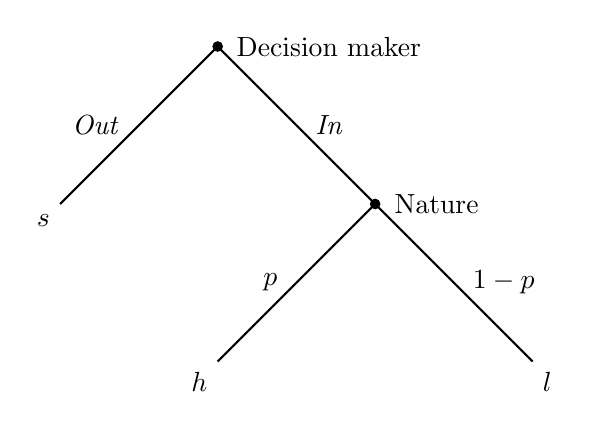
\begin{tikzpicture}[scale=2]
		\node[right] at (0,2) {~Decision maker};
		\draw[-, thick] (0,2) -- (-1,1) node[below left] {$s$};
		\node[left] at (-0.5,1.5) {\emph{Out}~~};
		\draw [fill] (0,2) circle [radius=0.03];
		\draw[-, thick] (0,2) -- (1,1) node[right] {~Nature};
		\node[right] at (0.5,1.5) {~\emph{In}};
		\draw [fill] (1,1) circle [radius=0.03];
		\draw[-, thick] (1,1) -- (0,0) node[below left] {$h$};
		\node[left] at (0.5,0.5) {$p$~~};
		\draw[-, thick] (1,1) -- (2,0) node[below right] {$l$};
		\node[right] at (1.5,0.5) {~$1-p$};		
	\end{tikzpicture}
\end{center}

In the following we look at different benchmarks.
In particular, we are interested in whether and how the optimal minimum acceptance probability $MAP^*$ depends on the distribution of $p$.


\subsection{Expected Utility Theory}
\label{subsec:EUT}

Assume the DM to have a utility function $U(\cdot)$. 
In an expected utility framework, utility is strictly increasing with outcome.
Hence, we have 
\begin{align}
	U(l) < U(s) < U(h)
\end{align}

The DM wants to choose his $MAP$ such that he maximizes his expected utility $U(MAP)$ which is
\begin{align}
	U(MAP) &= \int_{p=0}^{MAP} f(p) \cdot U(s) \, dp %%%
	+ \int_{p=MAP}^1 f(p) \cdot \left[p \cdot U(h) + (1-p) \cdot U(l) \right] dp \\
	     &= \int_{p=0}^{MAP} f(p) \cdot U(s) \, dp %%%
	     - \int_{p=1}^{MAP} f(p) \cdot \left[p \cdot U(h) + (1-p) \cdot U(l) \right] dp 
\end{align}

We use the Fundamental Theorem of Calculus to derive the first order condition:\footnote{
We have to say something here about SOC.
$\frac{\partial U}{\partial MAP} (0) > 0 $ and $\frac{\partial U}{\partial MAP} (1) < 0$ should do the trick.}
\begin{align}
	\frac{\partial U(MAP)}{\partial MAP} %%%
	= f(MAP) \cdot U(s) - f(MAP) \cdot \left[MAP \cdot U(h) + (1-MAP) \cdot U(l) \right] \stackrel{!}{=} 0
\end{align}

The density function $f(p)$ has full support.
Therefore, $f(p)$ is positive and we can simplify the expression to 
\begin{align}
	MAP^* = \frac{U(s)-U(l)}{U(h)-U(l)}
\end{align}

The optimal $MAP^*$ is independent of the distribution of $p$.
Thus, an expected utility maximizer should not be influenced by it. 


\subsection{Outcome Based Add-ons}

The result of Section \ref{subsec:EUT} holds if the utility function of the DM is extended by other elements that are based on outcomes.
For example, the DM might receive extra \mbox{(dis-)} utility from playing the lottery.
Or he might feel additional happiness or regret in case the outcome of the lottery is the high or the low outcome, respectively.
Such add-ons lead to a different $MAP^*$, but it remains independent of the distribution of $p$.  


\subsection{Probability Weighting}

Experimental evidence shows that humans have difficulties in handling probablities.
In particular, they seem to overestimate small probabilities.\footnote{
Some references would be nice here.
} 
In the following we assume the DM to have a continuous probability weighting function $w: [0,1] \rightarrow [0,1]$ with $w(0) = 0$ and $w(1) = 1$.
This gives the DM the following utility function:\footnote{
Probability weighting is not compatible with the axiomatic framework of expected utility theory.
We use the notion of utility in a broad sense covering also non-expected utility theories.
}
\begin{align}
	U(MAP) &= \int_{p=0}^{MAP} f(p) \cdot U(s) \, dp %%%
	+ \int_{p=MAP}^1 f(p) \cdot \left[w(p) \cdot U(h) + w(1-p) \cdot U(l) \right] dp
\end{align}

This leaves us with 
\begin{align}
	\label{eq:FOCsimplified}
	U(s) - \left[w(MAP) \cdot U(h) + w(1-MAP) \cdot U(l) \right] = 0 
\end{align}

From the assumptions about the weighting function and $U(l)<U(s)<U(h)$, it follows that this equation has at least one solution (Theorem of Bolzano).
As in Section \ref{subsec:EUT}, all solutions are independent of the distribution of $p$.\footnote{
We may get to a unique solution of equation (\ref{eq:FOCsimplified}) if we place additional requirements on the outcomes $U(\cdot)$ and/or on $w(p)$.
Two possibilities are:
1.) A unique solution is guaranteed if $w(p)$ is strictly increasing and symmetric, i.e. $w(1-p) = 1-w(p)$ or
2.) A unique solution is guaranteed if $w(p)$ is strictly increasing and the utility of the low outcome including all possible add-ons is set to zero, i.e. $u(b) = 0$.
}  
\footnote{
In case of multiple solutions we have to address that an individual might jump from one to the other solution depending on the distribution\dots
}
	


\subsection{Rank Dependent Utility}

Check \cite{Li2020a}.


\end{document}